\begin{pastexam}[label={px:ntut-109-ci-05}]{北科大資工所 109 學年度 第 4 題}
（簡答）

Given a set $S$ of characters (A, B, C, D, E, F, G, H, I) with relative frequencies (10, 5, 23, 18,
7, 12, 15, 4, 6). The \textbf{weighted path length} (WPL) is defined as $\Sigma$ ($f_i\times p_i$)
where $f_i$ is the frequency of character $i$ and $p_i$ is the length of the path in a code tree
from the root to character $i$. Let $T$ be an optimal Huffman code tree for $S$. Please answer the
following questions shortly. (5 pts)
\begin{enumerate}[label=(\arabic*)]
\item Is $T$ unique? (2 pts)
\item Do both characters B and H have the same path length from the root in $T$? (3 pts)
\end{enumerate}
\end{pastexam}

\begin{pastsoln}
答案：(1) 不唯一；(2) 是，B 和 H 的路徑長都是 $4$。

先照資結書第~19.3.4~節逐步建樹：每次取出頻率最小的兩個合併。 頻率由小到大是 H 4、B 5、I 6、
E 7、A 10、F 12、G 15、D 18、C 23，總和 $100$。
\begin{center}
\small
\begin{tabular}{clll}
\toprule
步驟 & 合併 & 新節點 & 合併後剩下的頻率 \\
\midrule
1 & H 4、B 5 & 9 & 6, 7, 9, 10, 12, 15, 18, 23 \\
2 & I 6、E 7 & 13 & 9, 10, 12, 13, 15, 18, 23 \\
3 & 9、A 10 & 19 & 12, 13, 15, 18, 19, 23 \\
4 & F 12、13 & 25 & 15, 18, 19, 23, 25 \\
5 & G 15、D 18 & 33 & 19, 23, 25, 33 \\
6 & 19、C 23 & 42 & 25, 33, 42 \\
7 & 25、33 & 58 & 42, 58 \\
8 & 42、58 & 100 & 100 \\
\bottomrule
\end{tabular}
\end{center}
每一步最小的兩個都是唯一的（第三小的都比第二小的大），整個過程沒有平手。 建出來的樹（較小的
放左邊）：

\begin{center}
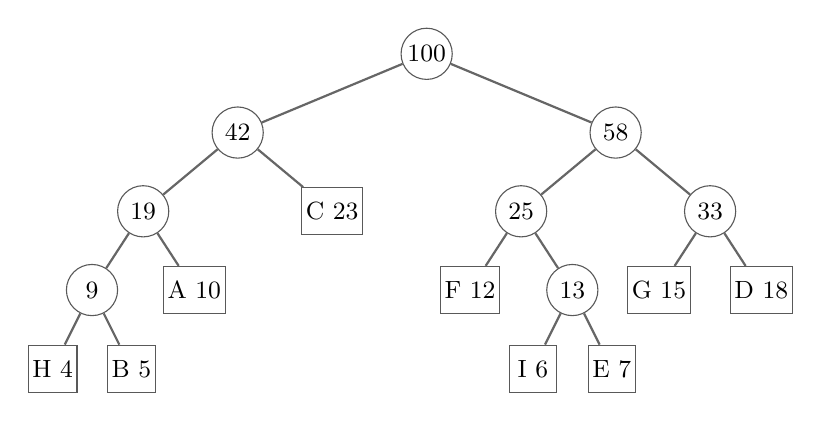
\begin{tikzpicture}[
    hn/.style={circle, draw=black!65, line width=0.4pt, minimum size=6.5mm, inner sep=0pt, font=\small},
    hl/.style={rectangle, draw=black!65, line width=0.4pt, minimum size=6mm, inner sep=1.5pt, font=\small},
    level distance=10mm, edge from parent/.style={draw=black!60, thick},
    level 1/.style={sibling distance=48mm}, level 2/.style={sibling distance=24mm},
    level 3/.style={sibling distance=13mm}, level 4/.style={sibling distance=10mm}]
\node[hn] {100}
    child {node[hn] {42}
        child {node[hn] {19}
            child {node[hn] {9} child {node[hl] {H 4}} child {node[hl] {B 5}}}
            child {node[hl] {A 10}}}
        child {node[hl] {C 23}}}
    child {node[hn] {58}
        child {node[hn] {25}
            child {node[hl] {F 12}}
            child {node[hn] {13} child {node[hl] {I 6}} child {node[hl] {E 7}}}}
        child {node[hn] {33}
            child {node[hl] {G 15}}
            child {node[hl] {D 18}}}};
\end{tikzpicture}
\end{center}

各字元的路徑長：C 是 $2$；A、D、F、G 是 $3$；B、E、H、I 是 $4$。
$\mathrm{WPL} = 23 \cdot 2 + (10 + 18 + 12 + 15) \cdot 3 + (5 + 7 + 4 + 6) \cdot 4 = 46 + 165 + 88 = 299$，
也等於所有內部節點的和 $9 + 13 + 19 + 25 + 33 + 42 + 58 + 100 = 299$。

\textbf{(1) 不唯一。} 每次合併兩棵子樹時，哪一棵當左子、哪一棵當右子可以任選，換了之後碼字不同、
WPL 一樣。 這裡有 $8$ 次合併，光是左右對調就有 $2^8 = 256$ 棵不同的最佳樹。 另外，同一層的兩片葉子
互換位置（例如 B 和 I 對調）也不改變 WPL，得到的也是最佳的前綴碼樹。 這組頻率在合併過程中沒有平手，
所以如果不管左右、只看合併的過程，霍夫曼演算法每一步的選擇是唯一的；但題目問的是樹 $T$，答
不唯一。

\textbf{(2) 是。} H（4）和 B（5）是頻率最小的兩個，而且第三小的 I 是 $6$，沒有平手，霍夫曼演算法第一步
一定合併它們，兩者在任何一棵霍夫曼樹裡都是兄弟，深度相同。 由上面的樹，兩者的路徑長都是 $4$。 這也
是資結書引理~19.3 說的：頻率最小的兩個字元可以是最深的一對兄弟。 （不只是霍夫曼演算法建出的樹：這組
頻率每一棵最佳前綴碼樹裡，各字元的深度都和上面相同，所以 B、H 一定同為 $4$。）
\end{pastsoln}
